\subsection{Stages of soot formation}

As shown in Fig.~\ref{fig:fv_growth_inception_dpm_timehis_comp}a, the optimized model reproduces the time evolution of $f_v$ measured using 1064~nm light extinction at 1984~K. The reported $f_v$ measurements are the average of values calculated using the min and max $E(m)$ of each wavelength. The predicted $f_v$ profile exhibits four distinct stages: (I) an initial period with negligible soot mass due to low inception and surface growth, known as the soot induction time, which is slightly overestimated by the model ($\approx$2.3~ms) compared to the measurements ($\approx$1.9~ms). A detailed discussion of induction time over the entire T$_5$ range is provided in Section~\ref{sec:tempeffect}. In stage (II), rapid growth occurs in $f_v$, driven by increasing PAH adsorption and HACA. The end of stage (II) signifies the inflection point in $f_v$, where both surface growth mechanisms reach their peak, as shown in Fig.~\ref{fig:fv_growth_inception_dpm_timehis_comp}b. At 1984~K, PAH adsorption is the dominant surface growth, accounting for nearly 79\% of total soot mass by 7.5~ms, and the rest ($\approx$21\%) originates from HACA. Inception is mainly active in stages (I) and (II), and its contribution to total soot mass remains less than 0.3\%. In stage (III), the increase of $f_v$ slows down due to the decline in both surface growth mechanisms. The time histories of $f_v$ and carbon yield, CY, are similar in the first two stages, but $f_v$ deviates from CY in stage (III). While $f_v$ gradually decreases at t$\approx$4.6~ms, CY gradually increases to reach 14.3\%. The decline of $f_v = V_{soot}/V_{gas}$ at $\approx$4.56~ms is attributed to gas-phase expansion caused by the arrival of the expansion wave at the endwall, reducing pressure (Fig.~\ref{fig:ptfv_pressure_type}a) and increasing $V_{gas}$ while $V_{soot}$ remains constant.

\begin{figure}[!t]
	\centering
	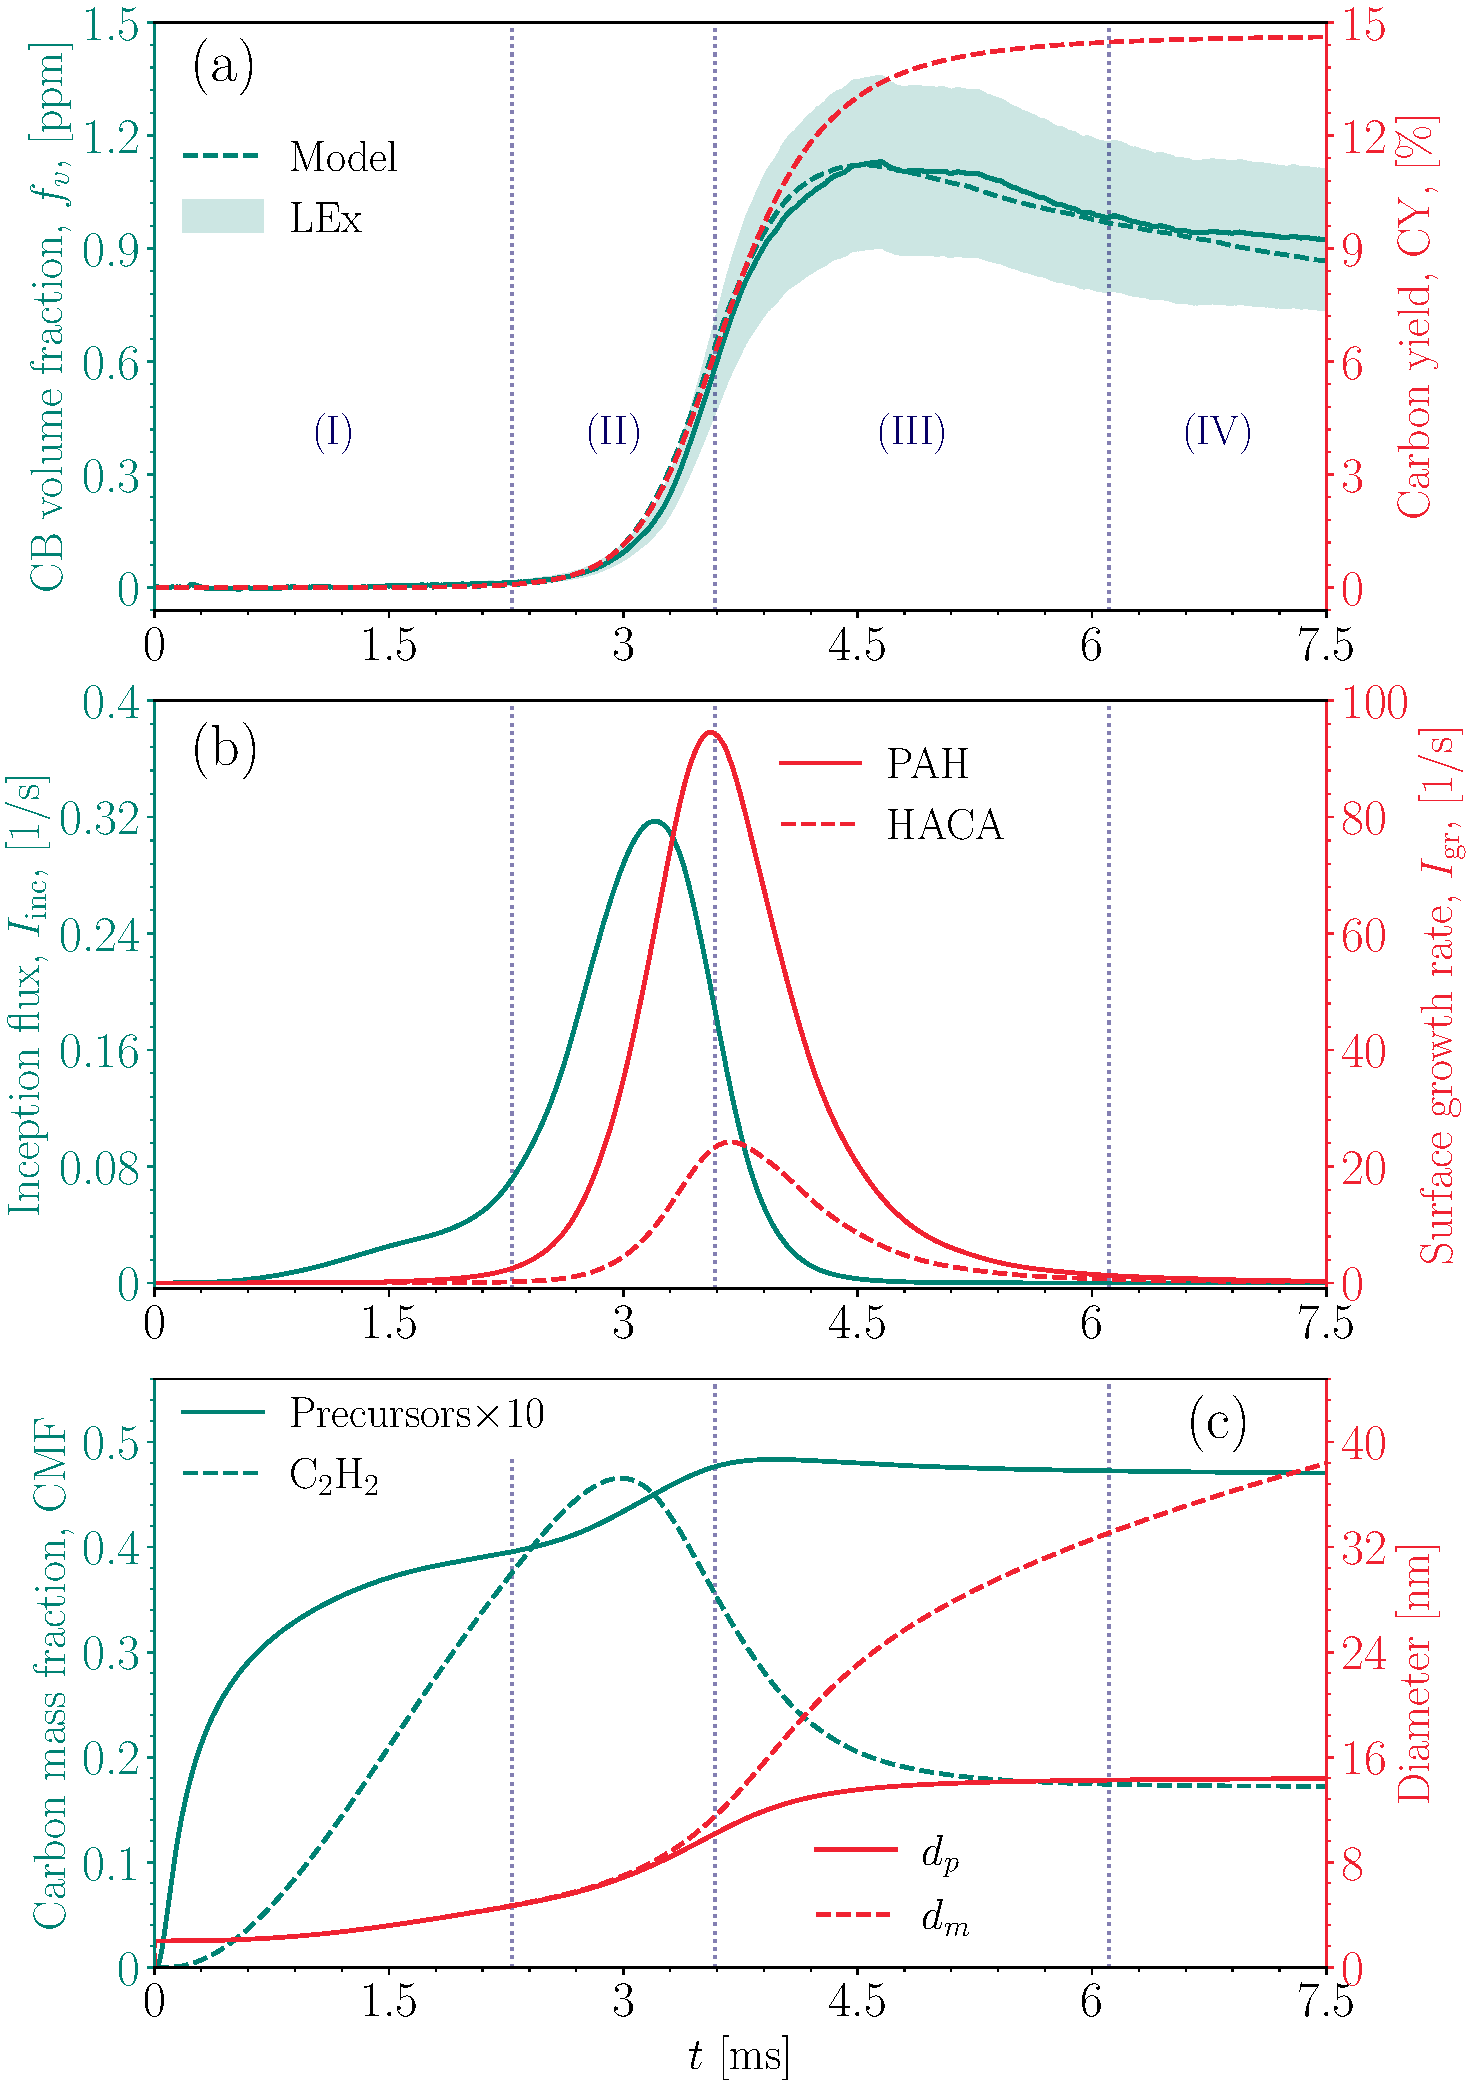
\includegraphics[width=0.65\textwidth]{Figures/Results/Paper3/fv_growth_inception_dpm_single.pdf}
	\caption{The four stages of soot formation demonstrated at T$_5$=1984~K for (a)  soot volume fraction, $f_v$, and carbon yield, CY (b) surface growth rate, $I_{\mathrm{gr}}$, via HACA and PAH adsorption, and inception flux; (c) the carbon mass fraction, CMF, of C$_2$H$_2$ and soot precursors combined, and primary particle diameter, $d_p$, and mobility diameter $d_m$, of soot agglomerates. Panel (a) depicts the light extinction measurements at $\lambda=1064$~nm with the shaded area representing the uncertainty from the variability in E(m).}
	\label{fig:fv_growth_inception_dpm_timehis_comp} 
\end{figure}


In stage (IV), surface growth rates become negligible, and soot agglomerates are chemically frozen, growing primarily through Brownian coagulation. As shown in Fig.~\ref{fig:fv_growth_inception_dpm_timehis_comp}c, soot morphology undergoes a corresponding transition. Here, $d_p$ and $d_m$ denote the average primary particle diameter and mobility diameter, respectively. These diameters remain identical until approximately 3~ms, near the peak of inception in stage (II), when most soot particles are spherical. Beyond 3~ms, the growth of $d_p$ slows and reaches 99\% of its terminal value of 14.4~nm before the end of stage (II) at approximately 5.89~ms, while $d_m$ continues to increase due to ongoing coagulation.

The rapid decline in inception rates (Fig.~\ref{fig:fv_growth_inception_dpm_timehis_comp}b) is primarily driven by the consumption of precursors through PAH adsorption, as evidenced by a factor of 2.3 decrease in their CMF between approximately 3~ms and 4.5~ms (Fig.~\ref{fig:fv_growth_inception_dpm_timehis_comp}c). Beyond 4.5~ms, PAH adsorption decreases as the temperature falls below 1600~K, which suppresses PAH dehydrogenation in the E-Bridge Modified model~\citep{adib2026omnisoot} and reduces the availability of PAH radicals for adsorption onto soot particles. Consequently, the CMF of precursors continues to decline after 4.5~ms and approaches 0.172 by the end of stage (III).

The reduction in HACA rates during stage (III) is mainly caused by a temperature-driven decrease in H radical concentration, which lowers the number of dehydrogenated surface sites, $\chi_{soot^{\circ}}$, in the HACA formulation~\citep{appel2000kinetic}. In addition, depletion of hydrogenated surface sites due to soot carbonization suppresses HACA rates throughout the simulation. Simulations performed without carbonization indicate an overprediction of the peak HACA rate by a factor of 2.4 and an overestimation of the final carbon yield by 46\%. While carbonization reduces the magnitude of the HACA rate, it does not affect the timing of its peak. Accordingly, the four stages identified in Fig.~\ref{fig:fv_growth_inception_dpm_timehis_comp} remain unchanged by carbonization.

\begin{figure}[!t]
	\centering
	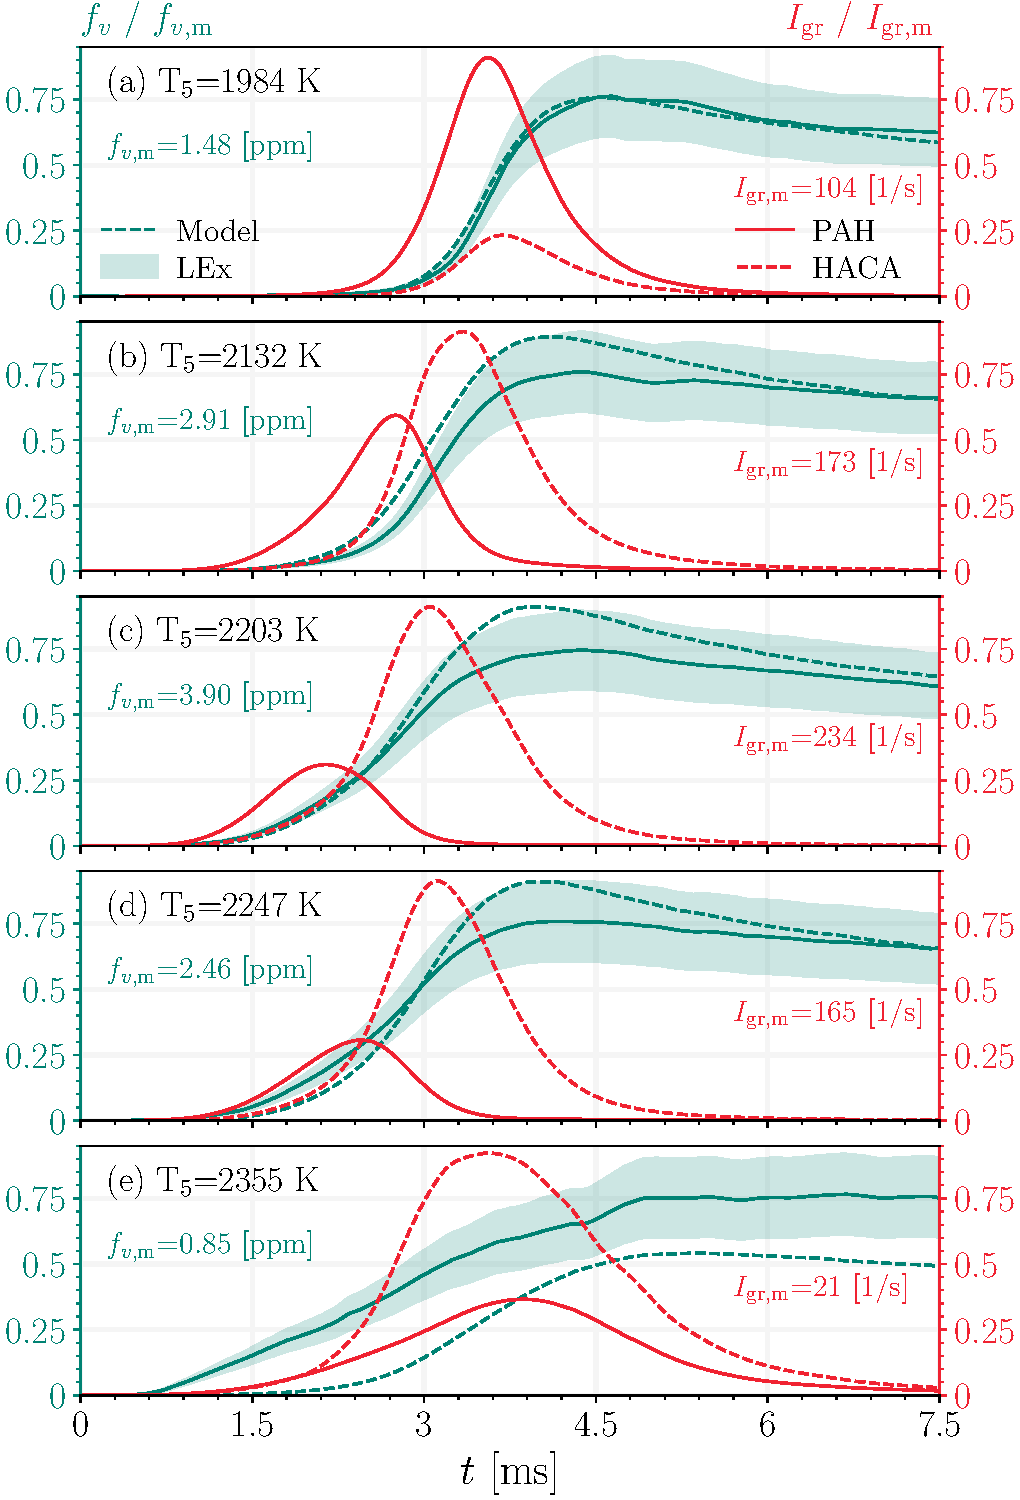
\includegraphics[width=0.65\textwidth]{Figures/Results/Paper3/fv_growth_five_cases.pdf}
	\caption{The time histories of normalized soot volume fraction, $f_v/f_{v,m}$ and normalized surface growth, $I_{gr}/I_{gr,m}$ at various temperatures. The measurements are from light extinction at $\lambda=1064$~nm with the shaded area representing the uncertainty from the variability in E(m).}
	\label{fig:fv_Igr_norm} 
\end{figure}

Fig.~\ref{fig:fv_Igr_norm} depicts the normalized soot volume fraction, $f_v/f_{v,m}$, and surface growth rate $I_\mathrm{gr}/I_\mathrm{gr,m}$ for the entire studied T$_5$ range. The time history of $f_v$ is predicted by the model for the entire T$_5$ range in good agreement with light extinction measurements, considering the sensitivity of $f_v$ to the pressure trace. The measured $f_v$ demonstrates that the onset of soot formation occurs earlier for higher T$_5$. In other words, stage (I) becomes shorter with increasing T$_5$. The model captures this shift from 1984~K to 2203~K, but noticeably predicts longer soot induction times at 2247~K and 2355~K compared to the measurements. The behavior of the model is dictated by precursor chemistry. PAH concentration has a bell-shaped temperature dependence with the peak at T$_5$=2203~K. Therefore, the inception and PAH adsorption rates decrease when T$_5$ increases to 2247~K and 2355~K.

HACA becomes the dominant surface growth mechanism for T$_5>$1984~K, as indicated by its higher peak compared to PAH adsorption. The analysis of integrated surface growth rates indicates that the contribution of HACA to the total carbon mass of soot increases from 21\% at 1984~K to 64\% at 2132~K and 77\% at 2203~K due to the increase in the inception flux producing more particles (active growth sites) and higher C$_2$H$_2$ concentration (Fig.~\ref{fig:CH4_C2H2_A2_A2R5_CRECK}b). However, the contribution of HACA slightly decreases to 75\% and 69\% for 2247~K and 2355~K, respectively, because the suppression of HACA by carbonization increases with temperature. Without carbonization, carbon yield reaches $\approx$100\% for T$_5\ge$2132~K with HACA accounting for more than 90\% of carbon mass.


\begin{figure}[!t]
	\centering
	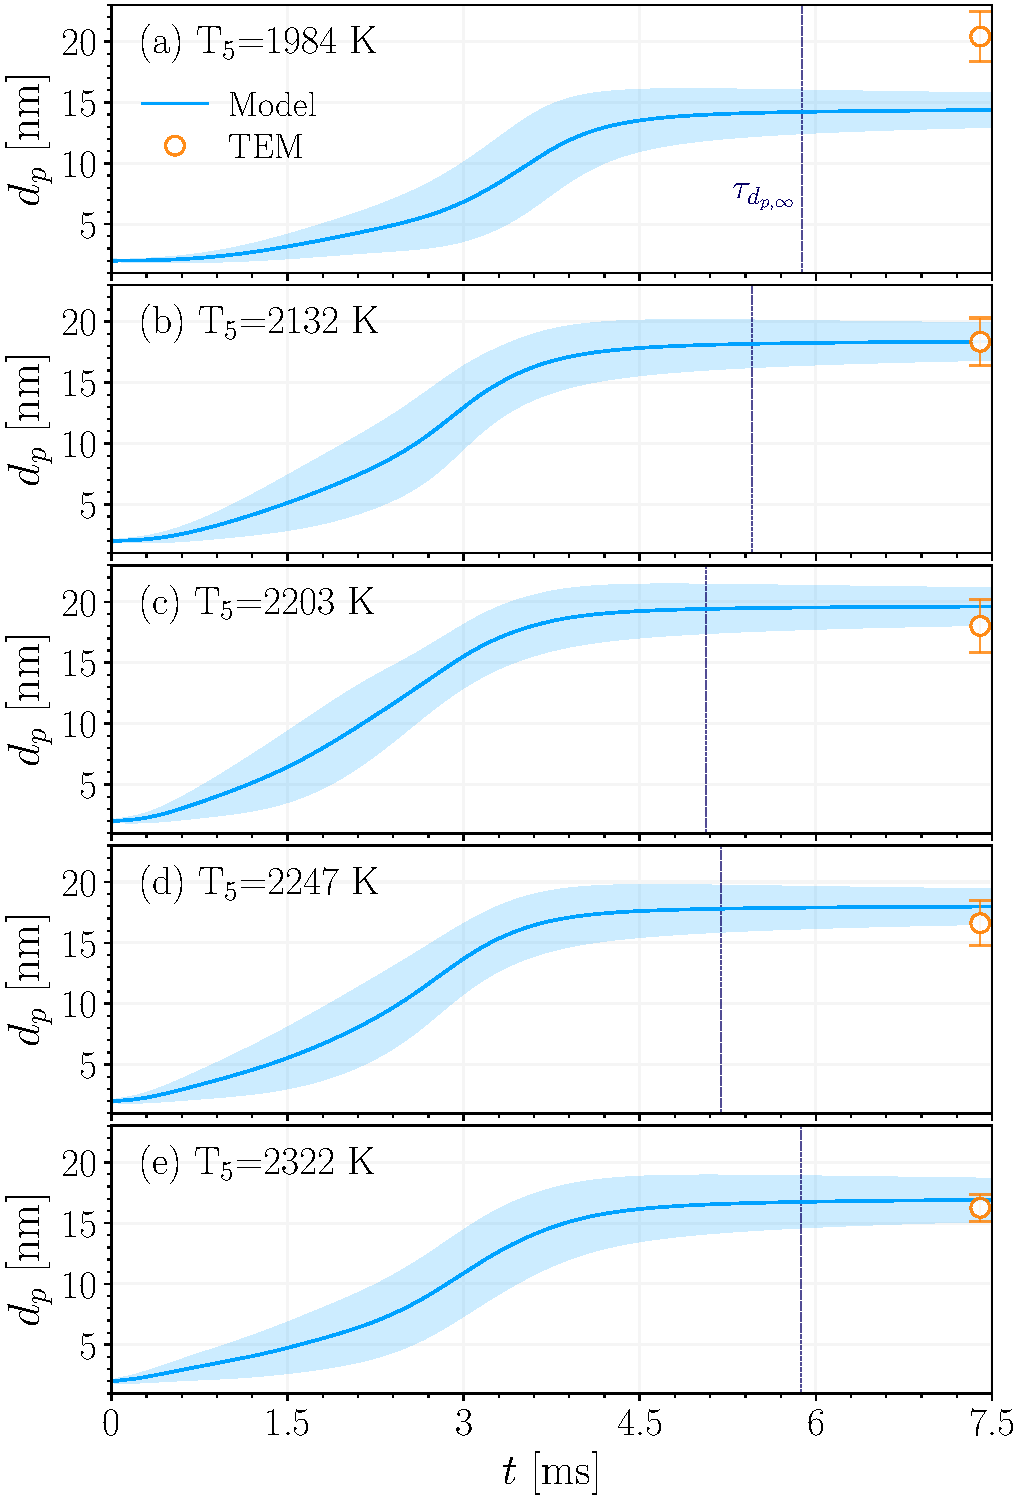
\includegraphics[width=0.6\textwidth]{Figures/Results/Paper3/dp_five_cases.pdf}
	\caption{The time histories of average primary particle diameter, $d_p$ compared with TEM measurement. The shaded area, and error bar represents the $d_p$ arithmetic standard deviation from the simulations and measurements, respectively. The dashed line specifies the time when $d_p$ reaches 99\% of its final value.}
	\label{fig:fv_dp_fivecases} 
\end{figure}

As shown in Fig.~\ref{fig:fv_dp_fivecases}, $d_p$ starts from 2~nm, which is the diameter of incipient soot defined in the model, increases through surface growth, and asymptotically approaches its final value, $d_{p,\infty}$. The characteristic time $\tau_{d_{p,\infty}}$, defined as the time at which $d_p$ reaches 99\% of $d_{p,\infty}$, remains below 6~ms for all T$_5$. These results indicate that no significant evolution of the primary particle diameter occurs beyond $\tau{d_{p,\infty}}$. Therefore, $d_p$ measured from collected TEM samples provides a representative measure of soot morphology within the studied time window. The predicted $d_{p,\infty}$ is in close agreement with the measurement, except for a noticeable underprediction at T$_5$=1984~K. $d{p,\infty}$ varies in a narrow range of 14-21~nm across various conditions. Primary particles have a relatively narrow size distribution; the standard deviation of $d_p$ increases due to persistent inception and surface growth, reaches a maximum of 3.8~nm, and finally converges to $\approx$1.5~nm. Table~\ref{tab:dp_tem_variousT5} lists arithmetic and geometric means and their corresponding standard deviations for the primary particle diameter computed from TEM measurements and model predictions. The difference between arithmetic ($d_p$) and geometric ($d_{p,g}$) remains less than 0.8\% across various conditions.

\renewcommand{\arraystretch}{1.2}
\begin{table}[!t]
	\centering
	\caption{The primary particle diameter measurements from TEM images. $d_{p}$ is arithmetic mean, $d_{p,g}$ geometric mean, $\sigma_{p}$ arithmetic standard deviation, and $\sigma_{p,g}$ geometic standard deviation.}
	\label{tab:dp_tem_variousT5}
	\begin{tabular}{l|ll|ll|ll|ll}
		\hline
		\multicolumn{1}{c}{} & \multicolumn{2}{c}{$d_{p}$~[nm]} & \multicolumn{2}{c}{$d_{p,g}$~[nm]} & \multicolumn{2}{c}{$\sigma_{p}$~[nm]} & \multicolumn{2}{c}{$\sigma_{p,g}$} \\ \hline
		T$_5$ {[}K{]} & TEM                   & Model        & TEM               & Model     & TEM                & Model       & TEM                  & Model       \\ \hline
		1984          & \textbf{20.4}         & 14.4         & \textbf{20.3}     & 14.3      & \textbf{2.1}       & 1.3         & \textbf{1.10}        & 1.10        \\ \hline
		2132          & \textbf{18.3}         & 18.4         & \textbf{18.3}     & 18.3      & \textbf{2.0}       & 1.5         & \textbf{1.11}        & 1.08        \\ \hline
		2203          & \textbf{18.0}         & 19.6         & \textbf{17.9}     & 19.6      & \textbf{2.2}       & 1.5         & \textbf{1.13}        & 1.08        \\ \hline
		2247          & \textbf{16.6}         & 18.0         & \textbf{16.5}     & 17.9      & \textbf{1.9}       & 1.4         & \textbf{1.12}        & 1.08        \\ \hline
		2322          & \textbf{16.3}         & 16.9         & \textbf{16.2}     & 16.8      & \textbf{1.1}       & 1.7         & \textbf{1.07}        & 1.11       \\ \hline
	\end{tabular}
\end{table}